\section{Setup}

This chapter demonstrate the how the testbed can be utilized in a specific scenario. First of all, the testbed requires users to define all the test cases in the \texttt{TEST} library. With the library, during the program uploading process, the specific device software would read the library and obtain some initial conditions much easier. Inside that library, users are supposed to construct schedule-lists for LBUs, and potentially action-lists for customized CPE behaviors. Both time division and end time should also be specified inside the library header file. The conditions of the spectrum, such as the number of the channel, the number of CPEs and LBUs in the test, should be specified in the \texttt{TEST} library as well. The testbed demonstration is designed to test with 1 BS, 5 CPEs, 3 LBUs to establish a single network region. The test will run for 1 week in virtual time, which translate to 15 minutes in real time.

Next, after setting up the testing stimulus, users should make sure the constant - ``operation'' = ``1'', running the experiment, in each of the programs: \texttt{base\_station.ino}, \texttt{customer\_premises\_equipment.ino} or \texttt{lisensed\_band\_user.ino}. Then, the programs are ready to be uploaded to the relevant devices. The project suggests that users use Arduino IDE to compile and upload all of the code. During the uploading process of LBUs and CPEs, even though each of these devices may need the same process code, it is important to assign unique ID names to them. Before uploading each one of LBUs and CPEs, be sure to change the ID that is located at the top of the ``.ino'' files. After all the uploadings, the devices will be ready to be launched. 

Before running the experiment, picking a location for the experiment is very important. All devices should be able to ``see'' each other at a distance, especially the BS. Try to find an open space where there is not much signal interference around the network operating frequency range. The demonstration that this paper explores picks an indoor location with each device separated two to three meters apart. The BS is located at the center of the region, and all the rest of the devices would just make a circle around it with a radius of approximately three meters. After the placement, a pre-test shows that they can clearly transmit or receive data from each other. This concludes the setup portion of the testbed experiment.

\section{Operation}

To begin the test, users need to turn on the devices one by one. First start with the BS, then the CPEs, and lastly the LBUs. For each CPE or LBU that is turned on, its blue LED will  first turn on and then off indicating a connection setup request has been sent into the air. The BS catches the connection request, responds to it and stores the corresponding client ID in the client-list. The blue LED from the CPE will turn on and stay on, indicating it is on ready state after receiving the response from the BS. If the blue LED turns off and stays off for a long time, that shows the initial connection has not been successfully established. In this case, this is probably due to weak signal in the area. Users should check the battery and try changing the location of the device. Then, simply launch the device to establish the connection again. The LBU connection process is the same as the one for CPE. The launching order doesn't matter within the same type of device. After the last LBU receives the connection indication, the BS should recognize that all devices are ready for the experiment. The BS will broadcast a ``start'' message to the air, so that every device receives and starts the program at the same time. All CPEs and LBUs turn off their lights at the same time, indicating they have received the broadcast at the same time. This is the initial synchronization process for the testbed.

During the experiment, the LEDs from the CPE flash, showing that the experiment is running perfectly. The demonstration runs for approximately 15 minutes. Within the time, one CPE may have a blue light on and the other CPE may have a yellow light on. This means the CPE with the blue light on is sending data to the CPE with yellow light on in a certain channel. The communication will go on for 5 seconds since the time division was set to 5 seconds for this demonstration. Sometimes the LEDs for a pair of communicating CPEs will suddenly black out during the 5 seconds. This is because the communication is interrupted by a LBU. After the communication is done, lights from the CPEs would also be turned off as they both go back to the requesting state. While all the successful communications and interruptions happen during the experiment, the occurrence counts are actually recorded by each individual CPEs. 

To output the result from the memory,the CPEs have to be given the memory outputting code. Simply change the defined variable ``operation'' to 2 at the beginning of \texttt{customer\_premises\_equipment.ino} file and upload to the CPE devices. As the device is turned on, it will run the memory outputting code. The Serial Monitor tool in Arduino IDE communicates with the device through SPI. When the individual device is connected to a client machine through USB, Arduino IDE can extract all the data inside Arduino EEPROM and print it to screen. Users can store the data for further process. If the experiment contains more than one trial, store the data this way after every trail, since the data would be erased and replaced by the new value from the next trial. This is what the operation process would look like. 

\section{Result and Discussion}

Determining if the testbed is a feasible tool for some of the algorithms out there could be broken down into the following ways: examining if the system operates normally and seeing if the output data expresses analytical value. The demonstration experiment mentioned in this chapter is designed to meet the two evaluation schemes. The same setup and operation runs four times, three with constant communication duration time, the other one with random communication duration time. Within the first three trials, they use different channel selection methods: first is in-order, second is random, third is with selection table. 

The methodology of the test relies on the assumption that channel switching is heavily affecting the performance of the system. With this assumption, there should be a linear relationship between performance and interruption count because each interruption requires a handoff or a channel switching, referring to the Figure~\ref{fig:channel_hopping}. When there are less interruptions, it implies that the network is utilizing the spectrum very well. Similarly, the more successful communication counts there are at the end of a trial, the better the algorithm it has. Therefore, the testbed is capable of accumulating the interruption counts, as well as the successful communication counts.

\begin{figure}[ht]
\centering
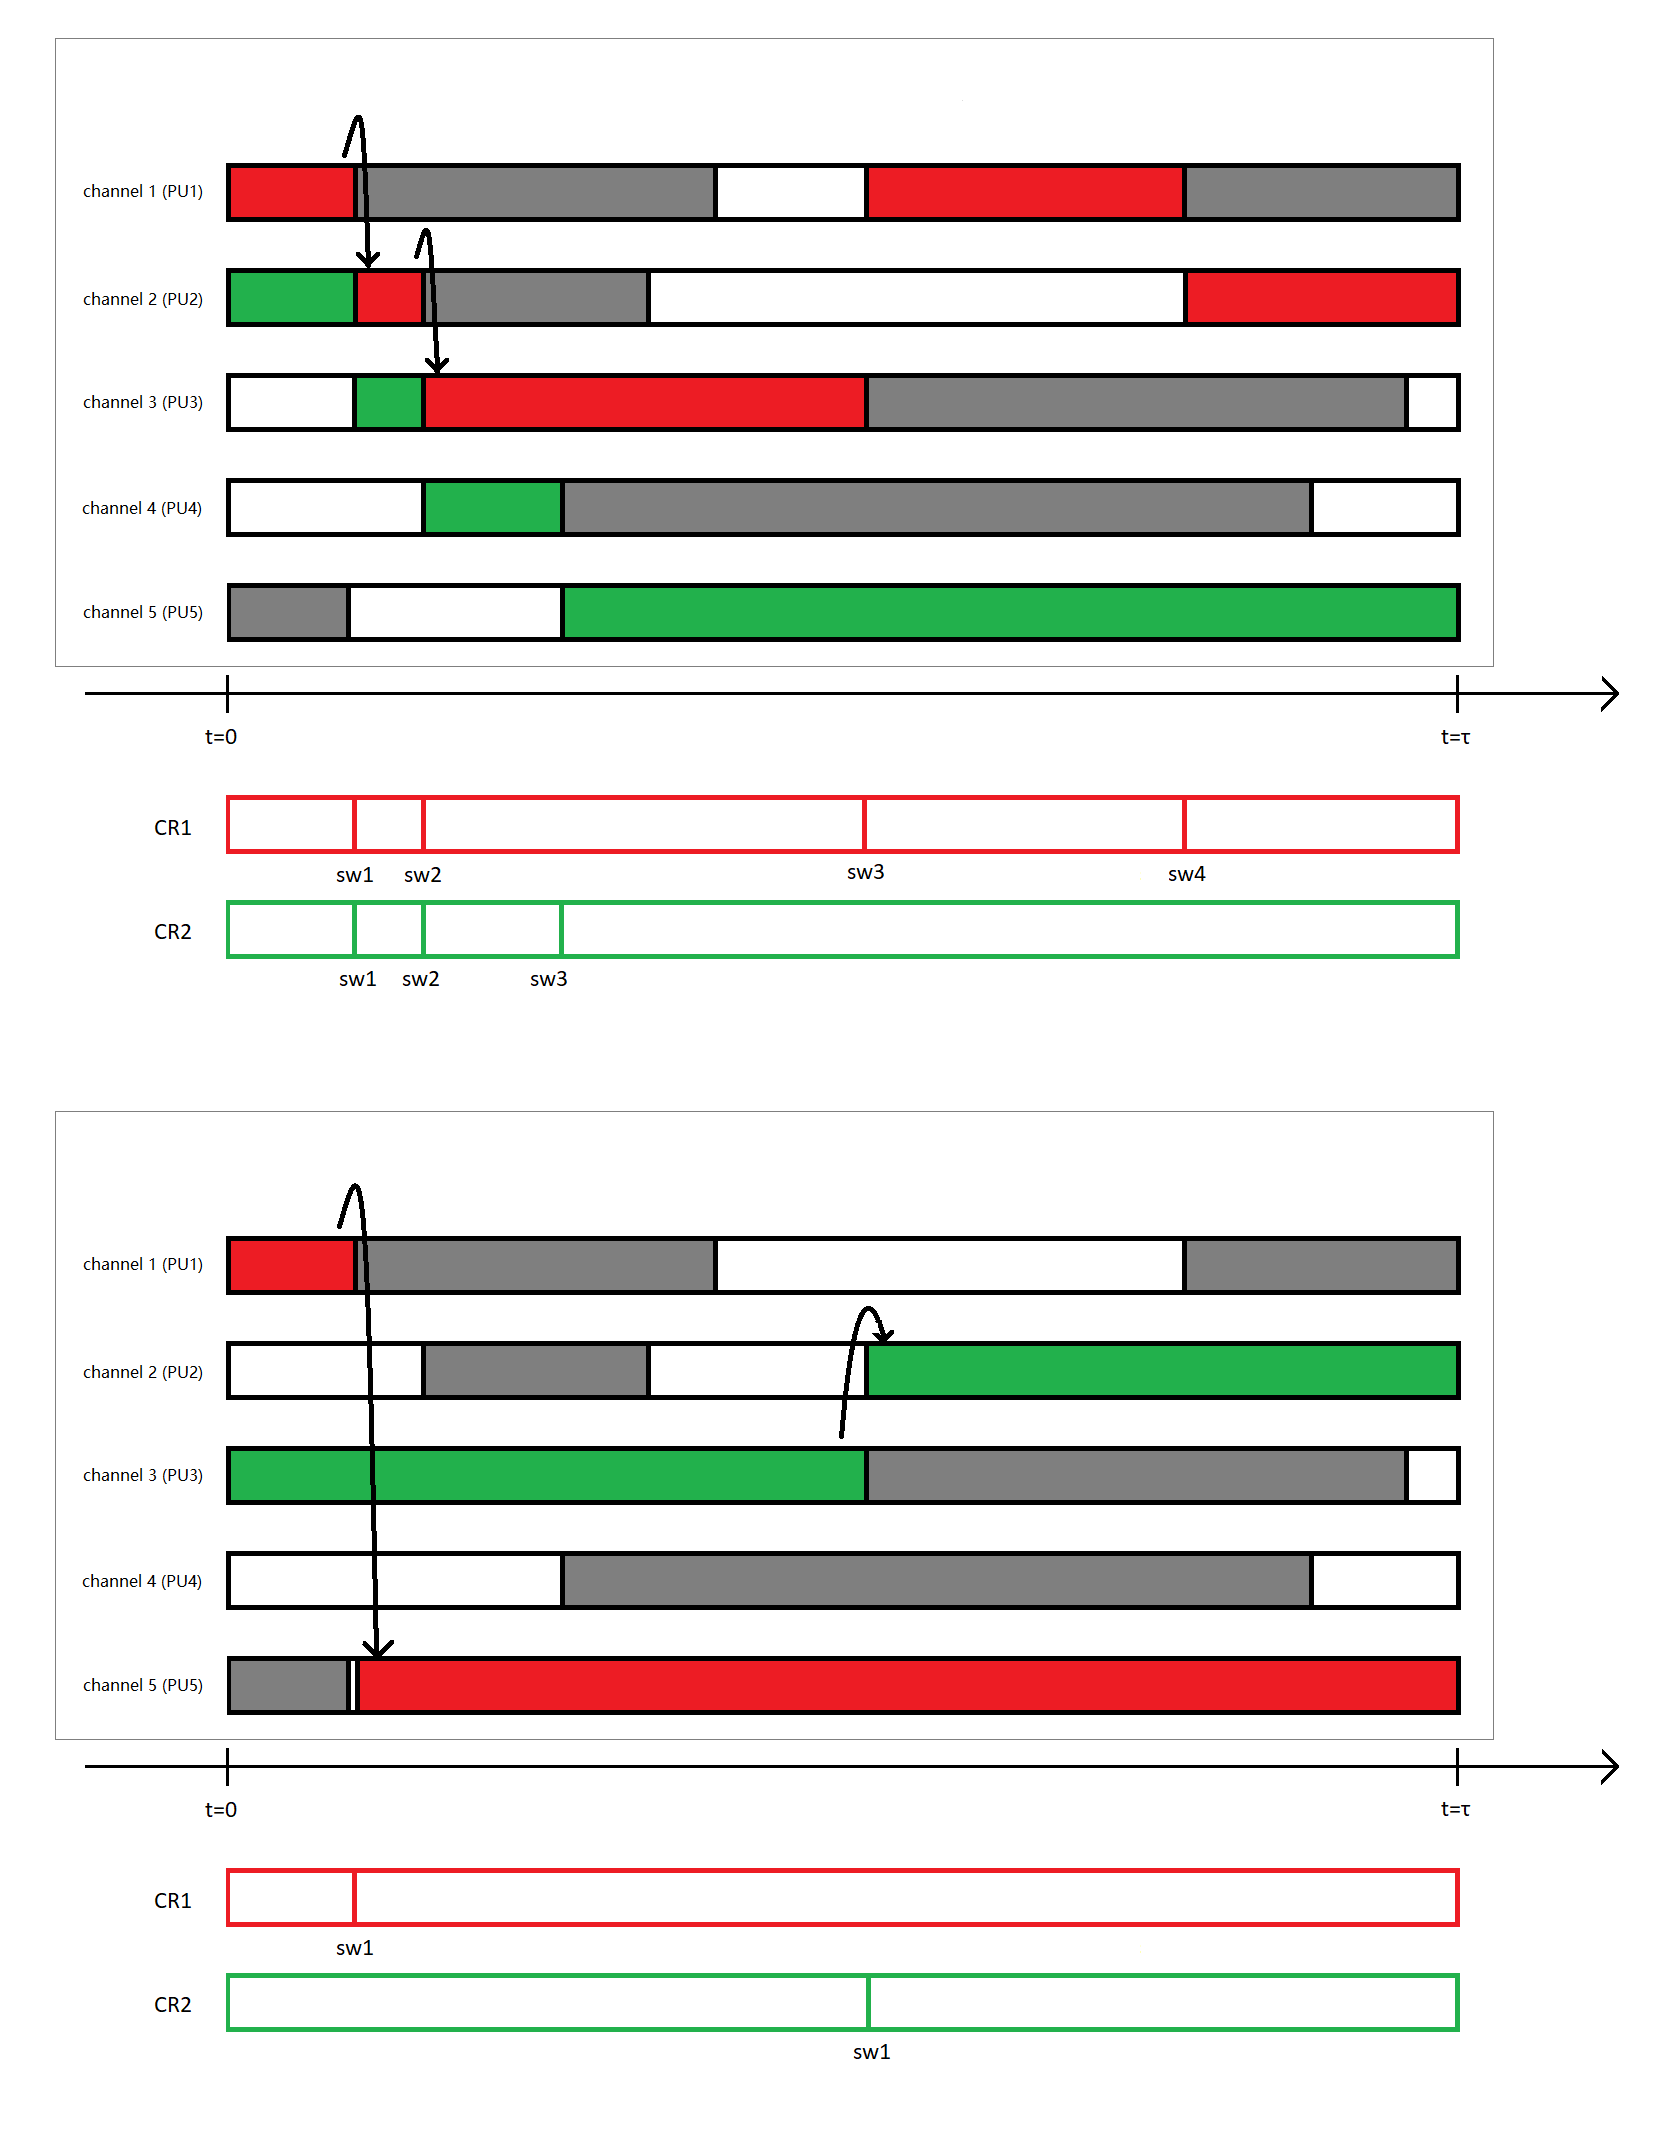
\includegraphics[width=10cm]{figures/channel_hopping.png}
\caption{Channel Hopping Comparison}
\label{fig:channel_hopping}
\end{figure}

The results show some interesting trends when comparing different channel selection algorithms and conditions. First, the comparison is represented in a bar graph shown in Figure~\ref{fig:performance_with_different_methods}. Here, it shows a graph of total transmission count across the same duration versus different channel selection choices. When using in-order selection, there are 131 transmissions without interruption within the 15 minutes of the trial. As it switches to random selection, a 140 success count is recorded. They have less than 10 percent of differences between the short 15 minutes. In theory, when the test stimulus signifies stochastic cases, there should not be any difference in choosing between the above two selection methods. Thus, the minor difference shown in the success transmission counts does not exemplify one method is superior than the other. However, the last trial has a significance of a 233 success transmission counts; it is approximately 60 percent more counts than the others. By simply adding a historical table (selection table) that keeps track of the spectrum usage, the system has a 1.6 times greater performance than the na\"ive logics. Figure~\ref{fig:interruption_in_a_week}(a) also illustrates a detailed interruption counts across the period of seven days in the trial. In-order and random channel selection methods shows a uniformly distributed data across the days. Yet, with the selection table inserted in the system, it shows trends of self-recognizing and self-learning during the process. After the first day with a lot of interruptions, it adapts and minimizes the interruptions, which is the key to maintain a high success transmission rate. In theory, since the test stimulus is designed to repeat every day, after the initial day, the system with historical data would have zero interruption for the rest of the time. Reasons for this remaining occurrence of interruption are both contributed by imperfection in the system logic and information delay during the update. With the result and knowledge of the system, users can have a rough evaluation of a channel selection algorithm.


\begin{figure}[ht]
\centering
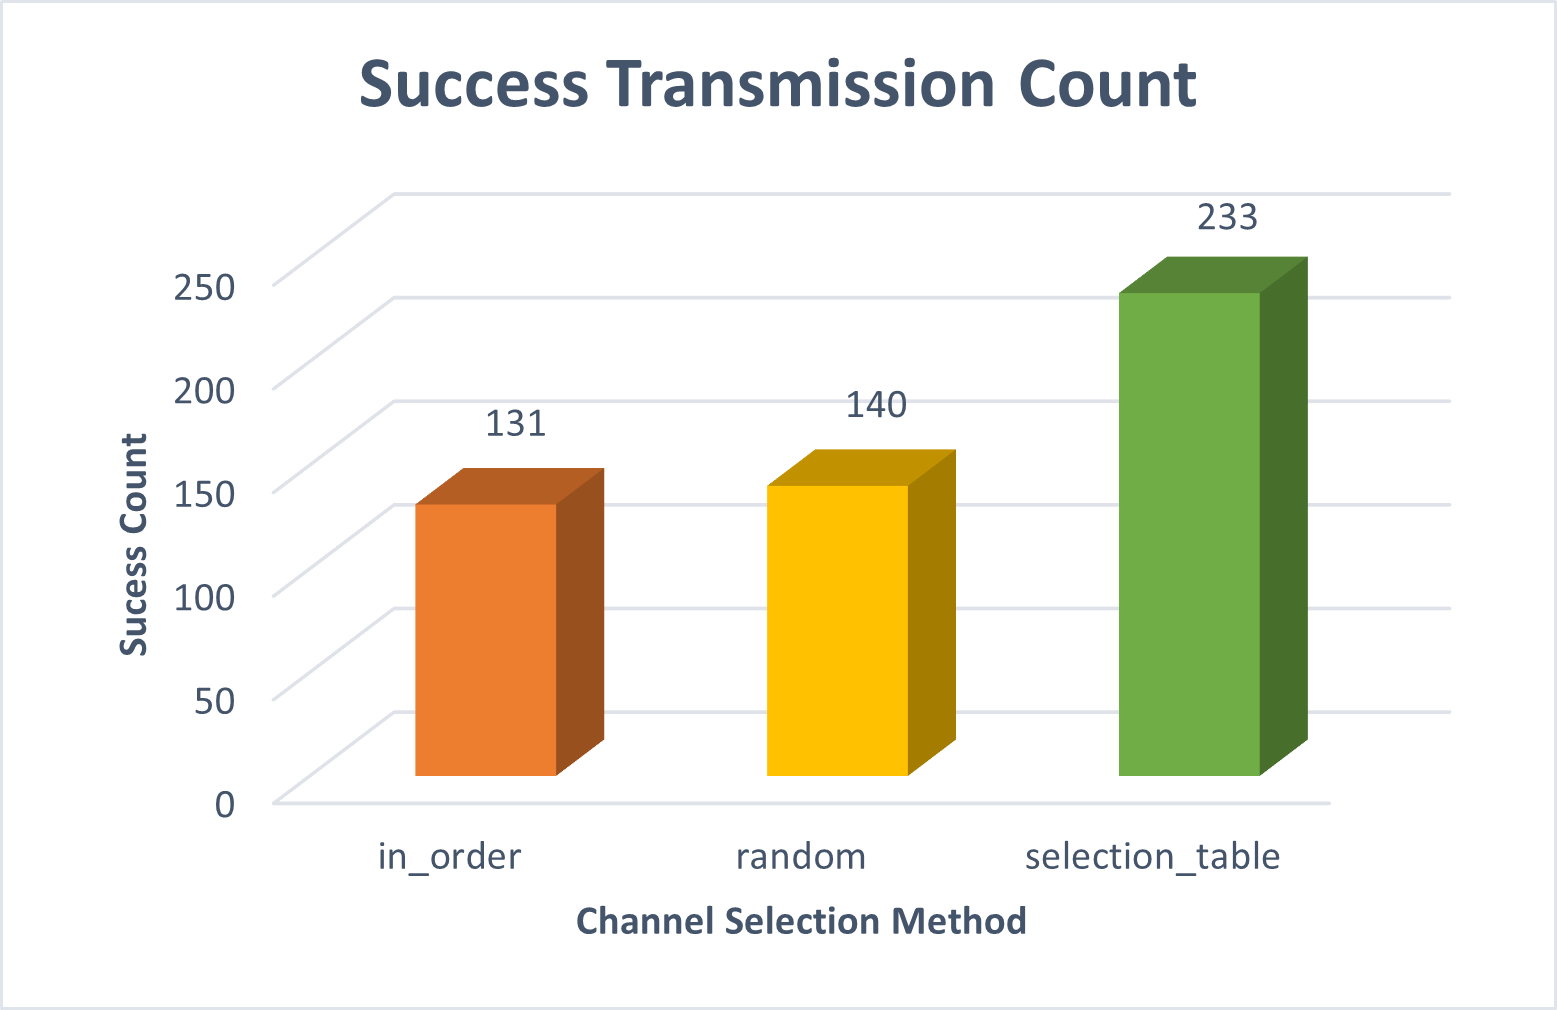
\includegraphics[width=10cm]{figures/total_success_count.png}
\caption{Over all Performance between Different Selection Methods}
\label{fig:performance_with_different_methods}
\end{figure}

Then, to push the system with selection table further, another trial is set up to test its capability to adapt to varying transmission time of the devices. As it shows in Figure~\ref{fig:interruption_in_a_week}(b), the divergence of the interruption count is not as great as the system that has a predicted transmission time. Yet, it demonstrates the trend of self-learning during the process as well. This kind of environment is also more appropriate when describing a real-life communication process, associating with an unpredictable communication duration. To accommodate different objects and regulations, users can tune the testing environment accordingly. To a certain extent, this testbed does represent the potential value of a proposal CR algorithm.

\begin{figure}[ht]
  \subfloat[Comparing Behavior with Different Selection]{
	\begin{minipage}[c][0.7\width]{
	   0.4\textwidth}
	   \centering
	   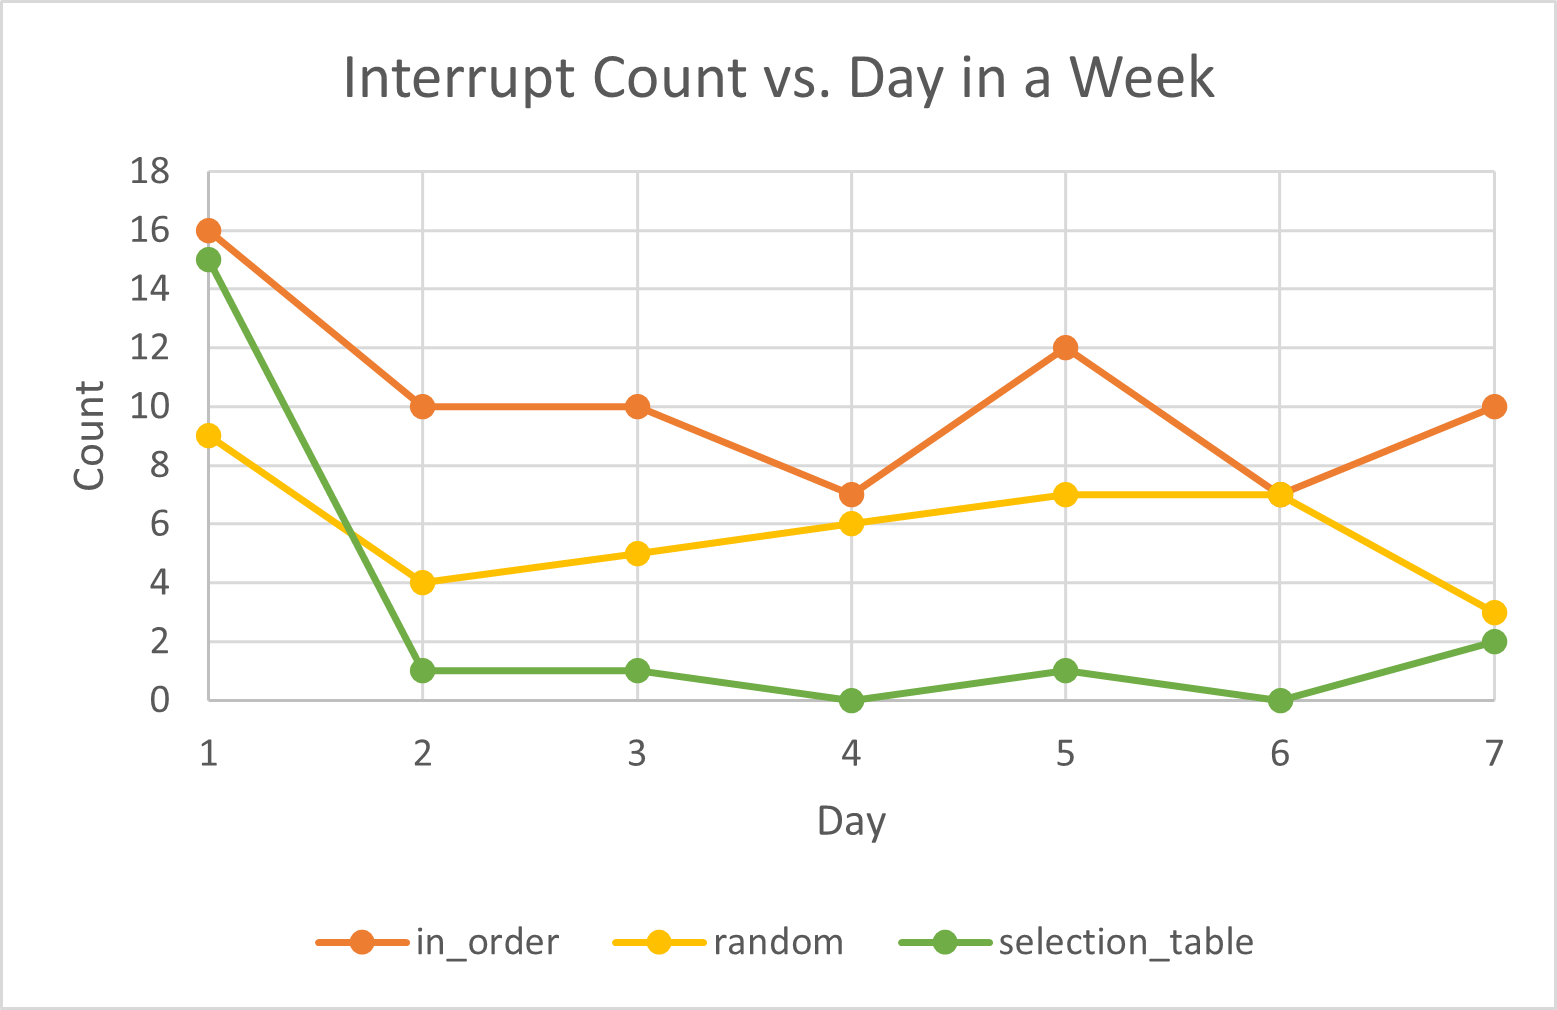
\includegraphics[width=1\textwidth]{figures/selection_comparison.png}
	\end{minipage}}
 \hfill 	
  \subfloat[Comparing Behavior with Different Duration Setup]{
	\begin{minipage}[c][0.7\width]{
	   0.4\textwidth}
	   \centering
	   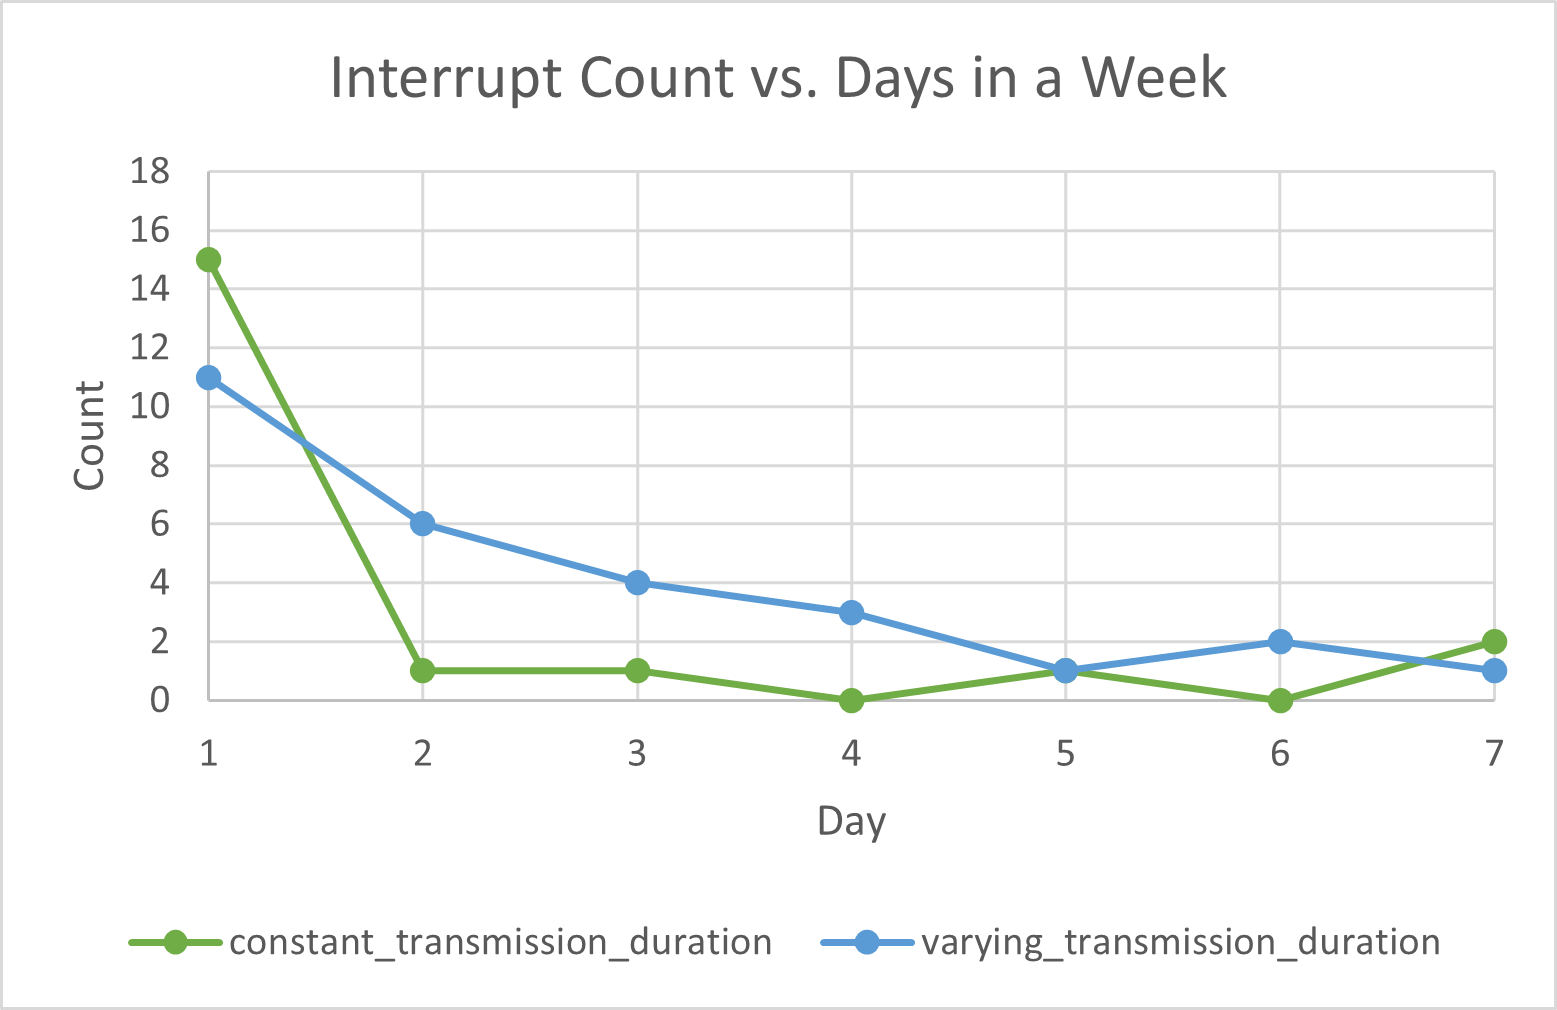
\includegraphics[width=1\textwidth]{figures/duration_comparison.png}
	\end{minipage}}
\caption{Interruption Counts across the Seven Days in a Week}
\label{fig:interruption_in_a_week}
\end{figure}
